%\documentclass[11pt, oneside]{article}   	
%\usepackage{geometry}    
%\geometry{letterpaper}                 		
\input preamble.tex
\newcommand{\ig}[2][width=4in]{\includegraphics[#1]{#2}}    		
\usepackage{graphicx}					
\usepackage{amssymb}
\usepackage{pgfplotstable}
\usepackage{float}
\usepackage{caption}
\captionsetup[table]{justification=justified,singlelinecheck=false, position=bottom}
\begin{document}

\header {\today}							
\title{Rutherford Scattering}
\author{Ekta Patel \& Brandon Booth-Dunbar}

\section{Abstract}
\begin{em} In this lab, we verify the Rutherford formula for nuclear scattering in 1909. Their experiment led to the confirmation of the existence of an atomic nucleus, thus destroying the plum pudding model  developed by J. J. Thomson. Rutherford's team successfully disproved Thomson's model by observing a significant amount of charged alpha particles scattering back from a thin sheet of gold foil rather than passing through it with only a few deflections. Therefore, they were able to confirm that an atom consists of a dense nucleus surrounded by a less dense cloud of electrons surrounding the heavy nucleus, instead of an even distribution of mass throughout the atom. The distribution of alpha particles scattered by gold foil can be observed as a function of the scattering angle, which relies on the distance between the foil and a detector. \end {em}

\section{Theory}
%B&E
Geiger and Marsden formed the first preliminary theory for the Rutherford model of the atom. They were able to gather that most $\alpha$-particles, He nuclei, passed right through a thin foil without being deflected. However, there were many particles that experienced large angle scattering. The differential scattering cross section will be determined in this lab: 
\begin{equation} \frac{d\sigma}{d\Omega}(\theta)\Delta\Omega=\frac{number\;of\; particles\; per\; unit\; time\;into\;a \;solid\; angle\; \Delta\Omega(\theta)}{(number \;of\; scatterers)\times (incident\; flux)} \end{equation}

Based on the previous definition, Rutherford was able to show that a positively charged nucleus has a differential scattering cross-section for charged particles that is given by:
\begin {equation}\label{scattering} \frac{d\sigma}{d\Omega}(\theta)= \frac{Z^2z^2e^4}{16E^2} \frac{1}{sin^4(\theta/2)}\end{equation} where $Ze$ is nuclear charge, $ze$ is charge of the scattered particle and $E$ is the energy of the scattered particle. $\theta$ is the scattering angle. However, we can see that this equation does not give appropriate units for a number of particles per area, instead we have $\frac{C^4}{J^2}$.
In order to correct this dimensional analysis disagreement, we look at the kinetic energy of the alpha particle, $E$, which is:
\begin{equation} E=\frac{1}{2}mv^2.\end{equation} However, when colliding alpha particles head on with the nucleus, all of the kinetic energy is turned into potential energy and the particle is at rest, so $E$ is also:
\begin{equation} E=\frac{q_1q_2}{4\pi\epsilon_0 b}.\end{equation} In the previous equation, $q_1=Ze$ and $q_2=ze$. We can solve for $b$, the distance between the center of the alpha particle and the center of the nucleus, where\begin{equation} b= \frac{Zze^2}{2\pi \epsilon_0 mv^2}.\end{equation}
Therefore, Equation \ref{scattering} can be rewritten as\begin{equation}\frac{d\sigma}{d\Omega}(\theta)=\left(\frac{1}{4b}\right)^2\frac{1}{sin^4(\theta/2)}.\end{equation}
\newline The scattering cross section can then be used to find the rate of detected particles, $N_2$, which is expressed in\ terms of $N_0$, the total number of particles emitted by the source per unit solid angle. Using the geometry of the set up and the Rutherford formula, the rate of detected particles is determined by the following formula
\begin{equation} N_2=n\frac{d\sigma}{d\Omega}(\theta)\Delta\Omega_2\times (incident\;flux)\end{equation} where $n$ is the number of scattering centers. The incident flux is given by $\frac{N_0}{R_1^2}$, which correspond to the figures in the next section. Then, $N_2$ is:
\begin{equation} N_2=\frac{nN_0}{R_1^2}\frac{d\sigma}{d\Omega}\Delta\Omega_2.\end{equation}
The scattering angle, $\theta$, varies with the changing distance $Y$ in the apparatus. Using the geometry of the setup, this formula can be given as
\begin{equation} \label{complicated}N_2=N_0\times \left( \frac{nA_2Z^2z^2e^4}{R_1^2r_1^2 16 E^2}\right)\times \left(\frac{cos\theta_2 sin\theta_2^2}{sin(\theta/2)^4}\right) \end {equation}\\or more simply as\begin{equation}  \label{simple}N_2=N_0\times G\times f(Y). \end{equation} Here G is the atomic factor that accounts for the force between the gold atoms and the scattered alpha particles as they pass through the gold foil. Here, we take for granted that the solid angles we mention are averages and that the scattering center is an average scattering center since we do not know where on the surface area of the gold foil each, or most, of the alpha particles will pass through. 
\section{Experimental Methods}
\subsection{Apparatus}
\begin{figure}[H]
\begin{center}
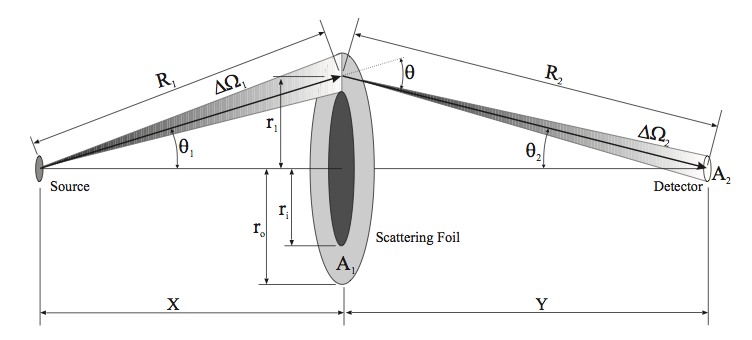
\includegraphics[width=7in]{apparatus.png}
\caption{Experimental geometry.}
\end{center}
\end{figure}
\subsection{Procedures}
\subsection{Calibration}
\subsection{Recording Data}

\section{Results and Discussion}
\subsection{The Scattering Angle Distribution}
Using Equations \ref{simple} and \ref{complicated}, solving the equation for $f(Y)$ gives the angular distribution as a function of Y. We can plot $Y$ vs. $f(Y)$ for a range of 0 cm to 20 cm to get a curve that we can use to fit our experimental results. We solve for f(Y) in the following steps:
\begin{equation} f(Y)=\frac{cos\theta_2 sin\theta_2^2}{sin(\theta/2)^4} \end{equation} where
\begin{equation} \theta_1=tan^{-1}\left(\frac{r_1}{X}\right)\end{equation} and
\begin{equation} \theta_2=tan^{-1}\left(\frac{r_1}{Y}\right)\end{equation} and
\begin{equation} cos\theta_2=\frac{Y}{\sqrt{Y^2+r_1^2}} \end{equation} and
\begin{equation} sin\theta_2^2=\frac{r_1^2}{Y^2+r_1^2}, \end{equation} therefore:
\begin{equation} f(Y)= \frac{\frac{Y}{\sqrt{Y^2+r_1^2}} \frac{r_1^2}{Y^2+r_1^2}}{sin(0.5(tan^{-1}\left(\frac{r_1}{X}\right) + tan^{-1}\left(\frac{r_1}{Y}))\right)^4.} \end{equation}\\
We know the following quantities as they are given in the lab manual because we cannot open the apparatus and check them for ourselves:
\begin{table}
\begin{center}
\begin{tabular}{|c|c|}\hline
Quantity & Description \\ \hline 
$r_s=0.32\pm0.01cm$ & radius of source\\ \hline 
$X=7.22\pm0.01cm$ & source to plane of scattering foil\\ \hline
$r_i=2.30cm$ & radius of the inside of the scattering foil\\ \hline
$r_o=2.70cm$ & radius of the outside of the scattering foil\\ \hline
$r_d=0.48cm$ & radius of the detector\\ \hline
\end{tabular}
\end{center}
\end{table}
Plotting this function for f(Y) over an interval of 0 to 20cm, we have:
\begin{figure}[h!]
\begin{center}
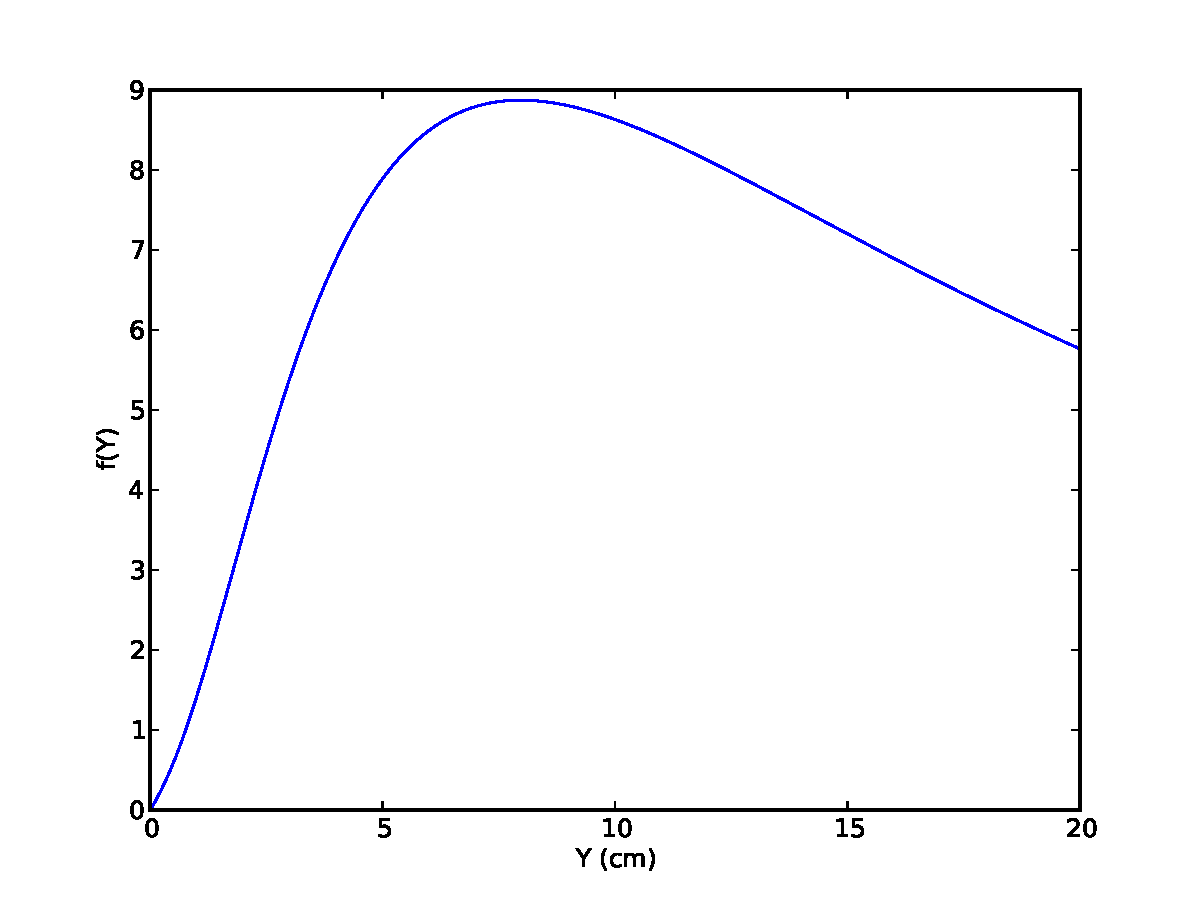
\includegraphics[width=4in]{preliminary_plot.pdf}
\caption{The angular distribution for the third term in the rate of detected particles($N_2$) that varies with the scattering angle as a function of length. The peak occurs in the vicinity of 8 cm.}
\end{center}
\end{figure}

\subsection{Determining $G$ \& $N_0$}
\begin{figure}[h!]
\begin{center}
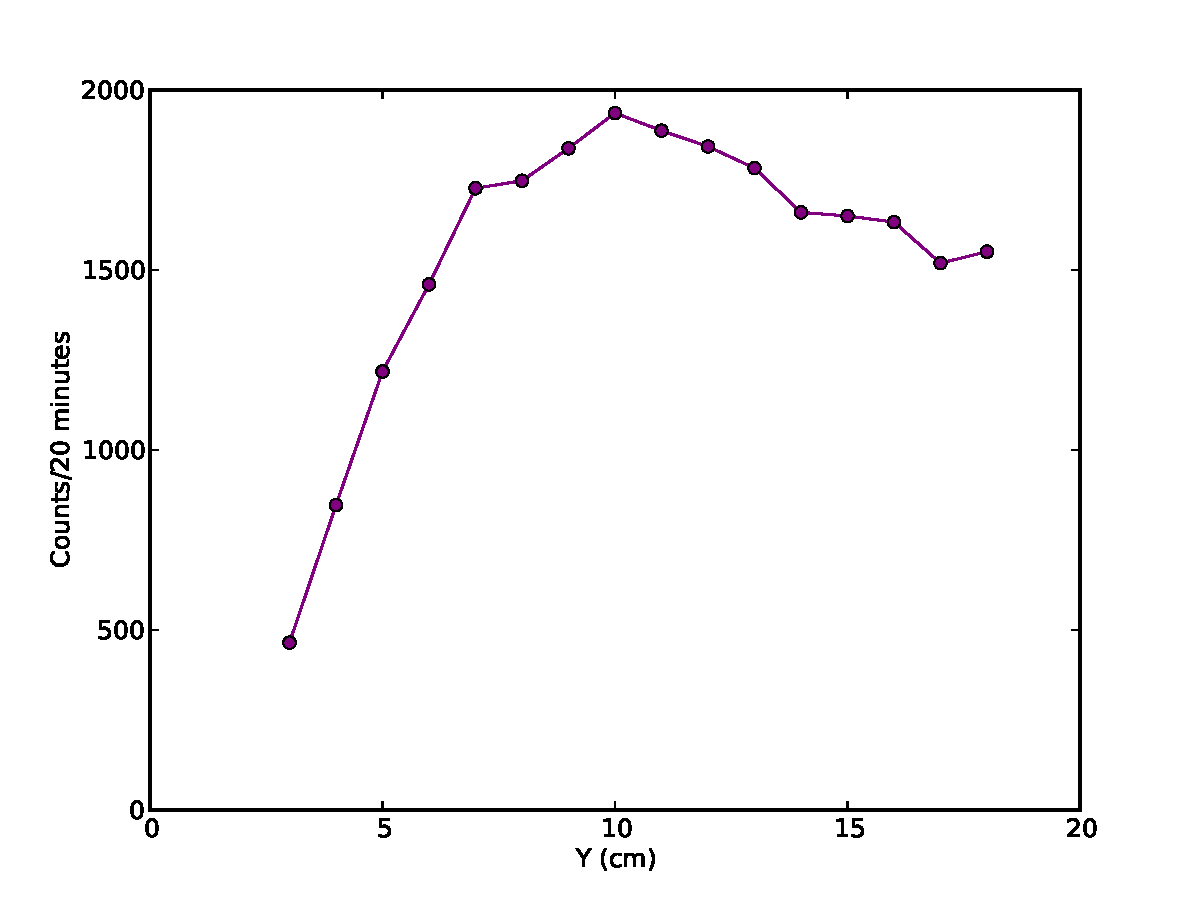
\includegraphics[width=4in]{firstrun.pdf}
\caption{The first run of data taken from 3cm to 18cm in intervals of 1cm.}
\end{center}
\end{figure}

\begin{figure}[h!]
\begin{center}
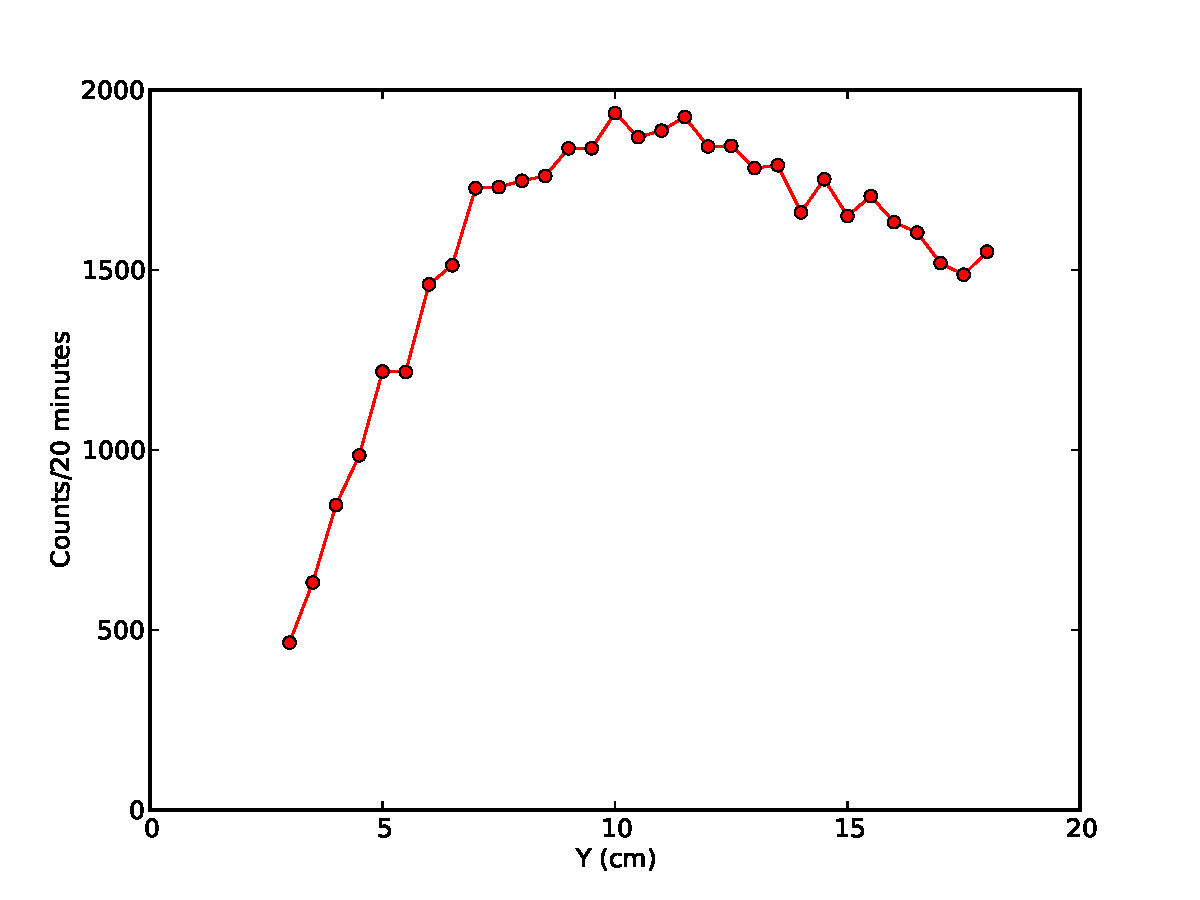
\includegraphics[width=4in]{secondrun.pdf}
\caption{The first run of data taken from 3cm to 18cm in intervals of 1cm with additional points taken in intervals of 0.5cm to obtain more statistics.}
\end{center}
\end{figure}
\subsection{Finding the Atomic Number ($Z$)}
\subsection{Calculating the Nuclear Radius Upper Limit}

\section{Conclusion}
%Brandon


\begin{thebibliography}{99}
\bibitem{electron}Sleator, Tycho, and Windt, David, \begin{em}Rutherford Scattering. \end{em}Experimental Physics. V85.0112. Spring, 2011.
\end{thebibliography}
\end{document}
